%2. serious game (play)
%- description of the game concept; goal(s) in the game
%- main elements in the game mechanics; game rules
%- essential feedback elements (in relation to the game goals)
%- challenges and dilemmas presented to the player
%- types of choices and actions available (and their role in relation to the game purpose)

In this chapter the game is explained in more detail. The game is designed to be engaging to support the real purpose as explained in chapter~\ref{chap:GamePurpose}. This chapter starts with the game story and an explanation of the game play. Subsequently the features of the game are explained. 

\subsection{Game Story}
The game starts with a story to get the user into the game. 
\\
\begin{wrapfigure}{l}{150px}
  \vspace{-30pt}
	\begin{center}
		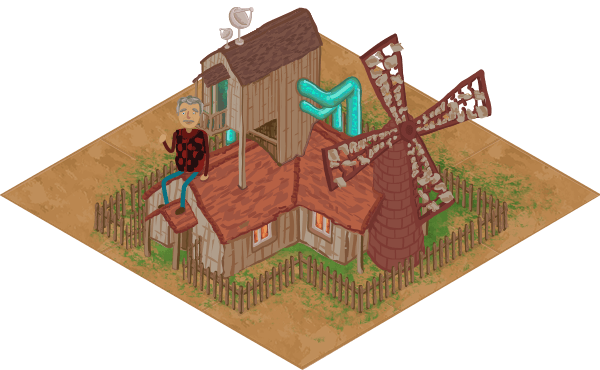
\includegraphics[width=150px]{images/farm.png}
	\end{center}
  \vspace{-10pt}
	\caption{The farm}
  \vspace{-20pt}
	\label{fig:farm}
\end{wrapfigure}
\textit{2542 AD. Your uncle was one of the first people to buy land in an unknown planet and decided to turn it into a farm to facilitate the earth's growing needs of food. Your uncle made the farm very profitable and he produced the best products available on earth. You received a mail telling you that your uncle had left you the farm already years ago. The fields on planet Yeo are unused and empty. Are you able to make the farm successful again?}
\\\\
\subsection{Gameplay}
The user is a novice farmer in the game and is instructed by a virtual physiotherapist, an old farmer called Phil. Phil instructs the user to learn and perform different types of exercises regularly that help to stay healthy in real life. Executing the exercises is also necessary to progress in the game. By cloning crops and livestock the user can become a more skilled farmer and revive the company. 
\\\\
The game mechanics are shown in Figure~\ref{fig:gameconcept}. The central point is the exercise, which influences all the progress in the game.

\begin{figure}[h]
	\centering
		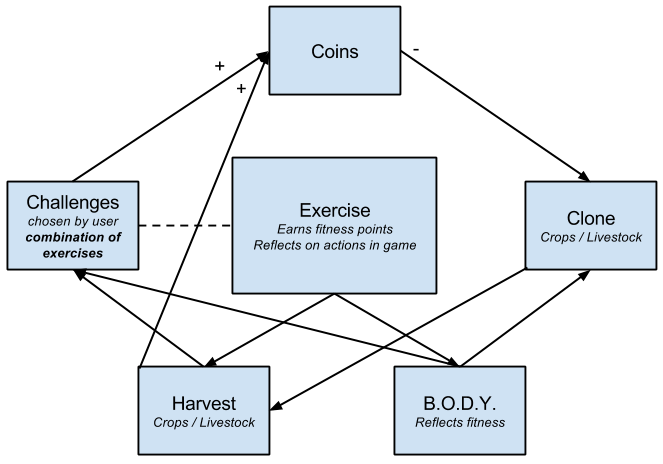
\includegraphics[width=0.80\textwidth]{images/gameconcept.png}
	\caption{Game mechanics}
	\label{fig:gameconcept}
\end{figure}

To clone crops or livestock on the farm, the farmer needs sufficient coins to buy them. Coins can be earned by harvesting products or by completing challenges. The user can pay coins to clone the crops or livestock and place them on tiles in the map. In a certain time interval the crops are ripe and can be harvested and livestock products can be gathered. In order to do this, specific exercises are to be executed in real life. 
\\\\
Challenges are separate stories and require the execution of a set of exercises focused on a specific body region or on the full body. Most of the challenges require you to harvest some items before starting them.
\\\\
The farmer is equipped with a Bionic Outer Dimension Yeosuit (B.O.D.Y.) as described in chapter \ref{chap:GamePurpose}. The B.O.D.Y. reflects all the exercises the user has executed. For example, after performing an exercise that focuses on chest muscles, experience points are added to the B.O.D.Y. for the chest. Once the user has enough experience points for each body part, the level of the B.O.D.Y. is increased. This way, the user is informed about which body regions have to be improved and need more focus in the future. An upgrade of the level of the B.O.D.Y. allows the user to clone more products and unlocks new challenges.
\\\\
More details about each of these components will be given in paragraph~\ref{subsec:GameFeatures}.

\subsection{Example game scenario}
This section provides an example of the game play. In this example, the user clones a space apple tree with his money and plants it on any available tile on the map. After a few hours the apples can be harvested, additionally the user can request for a notification to be informed. To harvest the apples, the user has to execute an exercise for picking apples. The mentor gives a description of the exercise in detail and also show how to execute the exercise properly for the users less interested in reading the description. Once the apples are harvested, the user receives the corresponding reward in coins and the harvested space apples are added to the inventory. These space apples might be used to start new challenges or feed the Piggiums, the cloned pigs that are exported to space.

%--List of features explained--
\subsection{Game features}
\label{subsec:GameFeatures}
The sections below describe all game features and their specifications more extensively. This may differ from the original game design document, as several features were left out of the game for varying reasons. These will be discussed in paragraph~\ref{sec:FutureWork}.

\subsubsection{The overview}
At the start of the game, the user sees an introductional story before the farm is shown. A short explanation of the game is given and the B.O.D.Y. is introduced to make the purpose of the game clear. After these introductions the player is ready to start his adventure.
\\\\
Now the farm will be introduced to the user and the uncle is awaiting him there. The amount of space around the farm is fixed throughout the duration of the game. The user is asked by Phil to clone a crop, harvest the crop and finish a challenge. After doing these tasks the user has explored the most important features of the game and should be able to continue without further help. From now on, Mentor Phil provides the user with a daily task to help aiming for a healthy lifestyle. 
\\\\
A screenshot of what the map looks like is shown in Figure~\ref{fig:map}.

\begin{figure}[h]
	\centering
		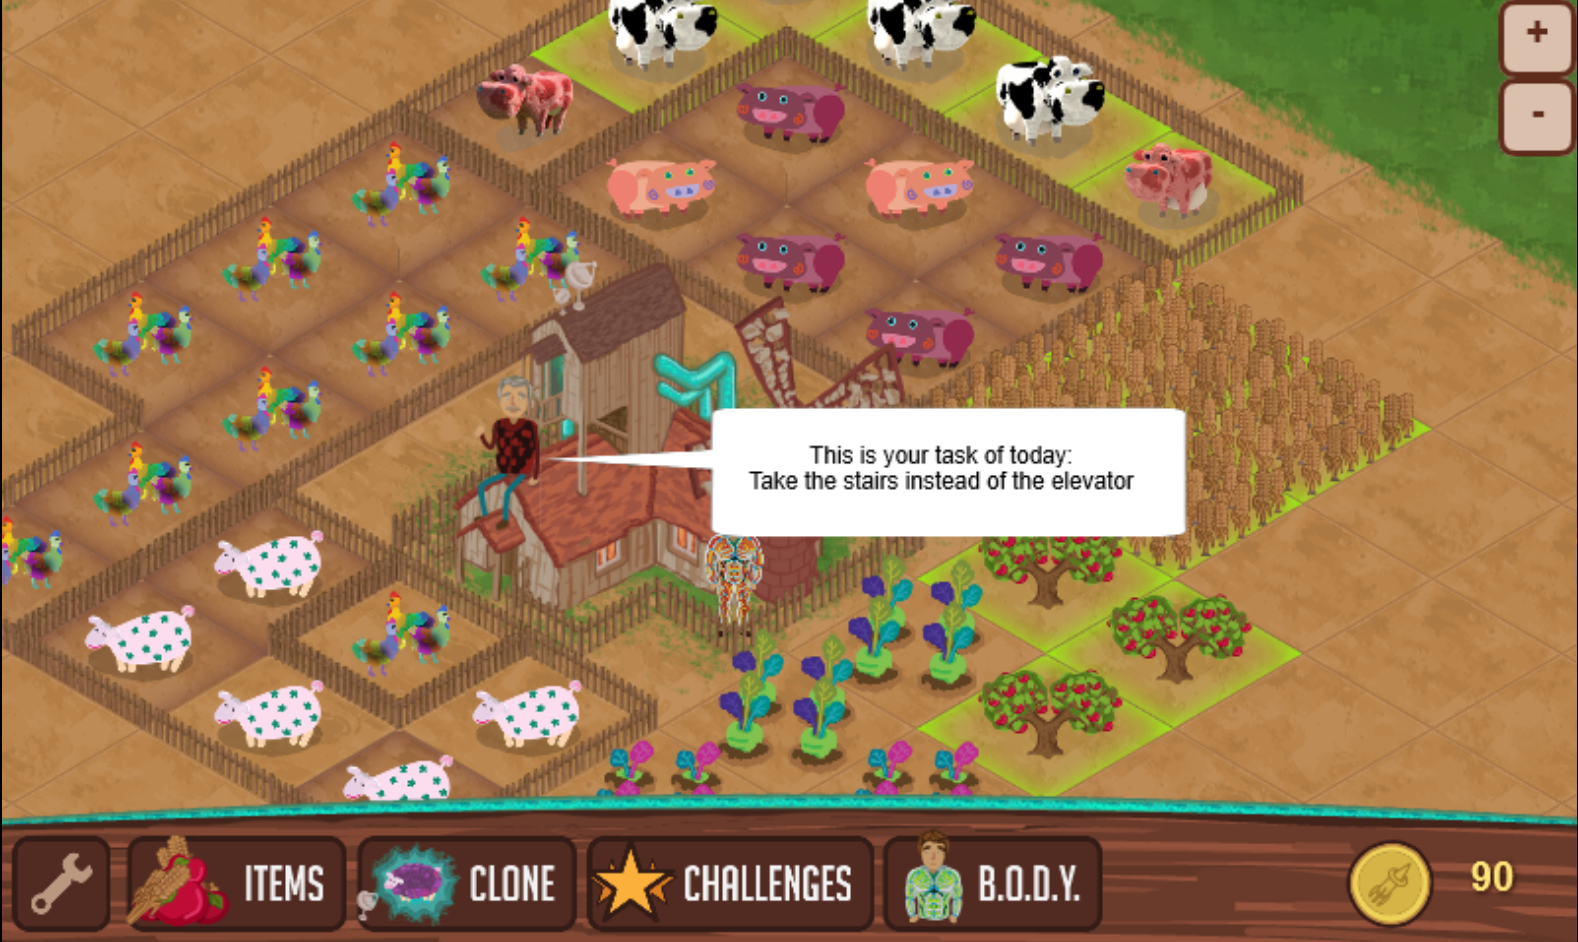
\includegraphics[width=0.80\textwidth]{images/map.png}
	\caption{The map overview}
	\label{fig:map}
\end{figure}

\subsubsection{Mentor Phil}
Once you get to the farm, you discover there is a very old friend of your uncle's, Phil, who is around 60 years old, but still very much in shape. He will serve as your mentor and "personal coach" in the game. Phil explains the purpose and shows the correct execution of each exercise to you. During the game, the mentor and the player will become friends and ``partners in exercise''.

\subsubsection{The farmer}
In the game, the player is impersonated by a farmer. The farmer wears the B.O.D.Y. which is upgraded according to the performed exercises.

\subsubsection{Bionic Outer Dimension Yeosuit}
Apart from the advice part that the player gets from Phil, he also gets reflection of his progress in the game in the form of a ``B.O.D.Y.''. The player has a list of points, one for each body part (arms, legs, abs, back, chest), and each finished exercise will yield some points for a specific body part. When the points for each body part have reached a certain amount, the player is awarded an upgrade of the level of his B.O.D.Y. The upgrade depends on the body part with the least experience points (a chain is as strong as its weakest link). This way, the player will notice when he's focusing too much on one or several body parts and will be motivated to also focus on the other parts. Now the player has a choice in the exercises he performs, but is motivated to make a balanced scheme. 
\\\\
The level of the player is defined by the progress of the B.O.D.Y. In this way, the B.O.D.Y. gives an indication of the progress in the game and the physical performance.  A higher level gives the player more skills and unlocks new crops and livestock.
\\\\
A screenshot of what the B.O.D.Y. looks like is shown in Figure~\ref{fig:body}. As you can see in this image, the player is somewhat behind on his back exercises.

\begin{figure}[h]
	\centering
		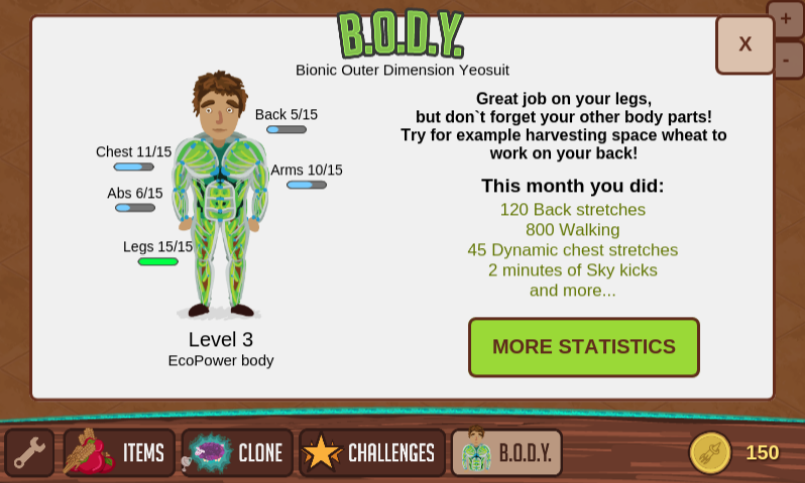
\includegraphics[width=0.80\textwidth]{images/SceneBody.png}
	\caption{The B.O.D.Y.}
	\label{fig:body}
\end{figure}

\subsubsection{Exercises}
During the game, players are asked to execute several exercises in real life. These exercises are necessary for them to harvest a crop, or to exploit the livestock. Prior to each exercise a clear explanation is shown about the movement the player has to perform demonstrated by a drawing of the mentor. The phone is used to measure the execution of the exercise and is handheld by the player. The accelerometer of the phone measures the movement. There are also exercises in the challenges, which are described in the next section. Most of those exercises are measured by a stopwatch, trusting the player's own motivation to execute them correctly. After completing an exercise, the player will be informed which body parts he has exercised by an overview of how much the B.O.D.Y. has improved.
\\\\
A screenshot of what an active exercise looks like is shown in Figure~\ref{fig:exercise}.

\begin{figure}[h]
	\centering
		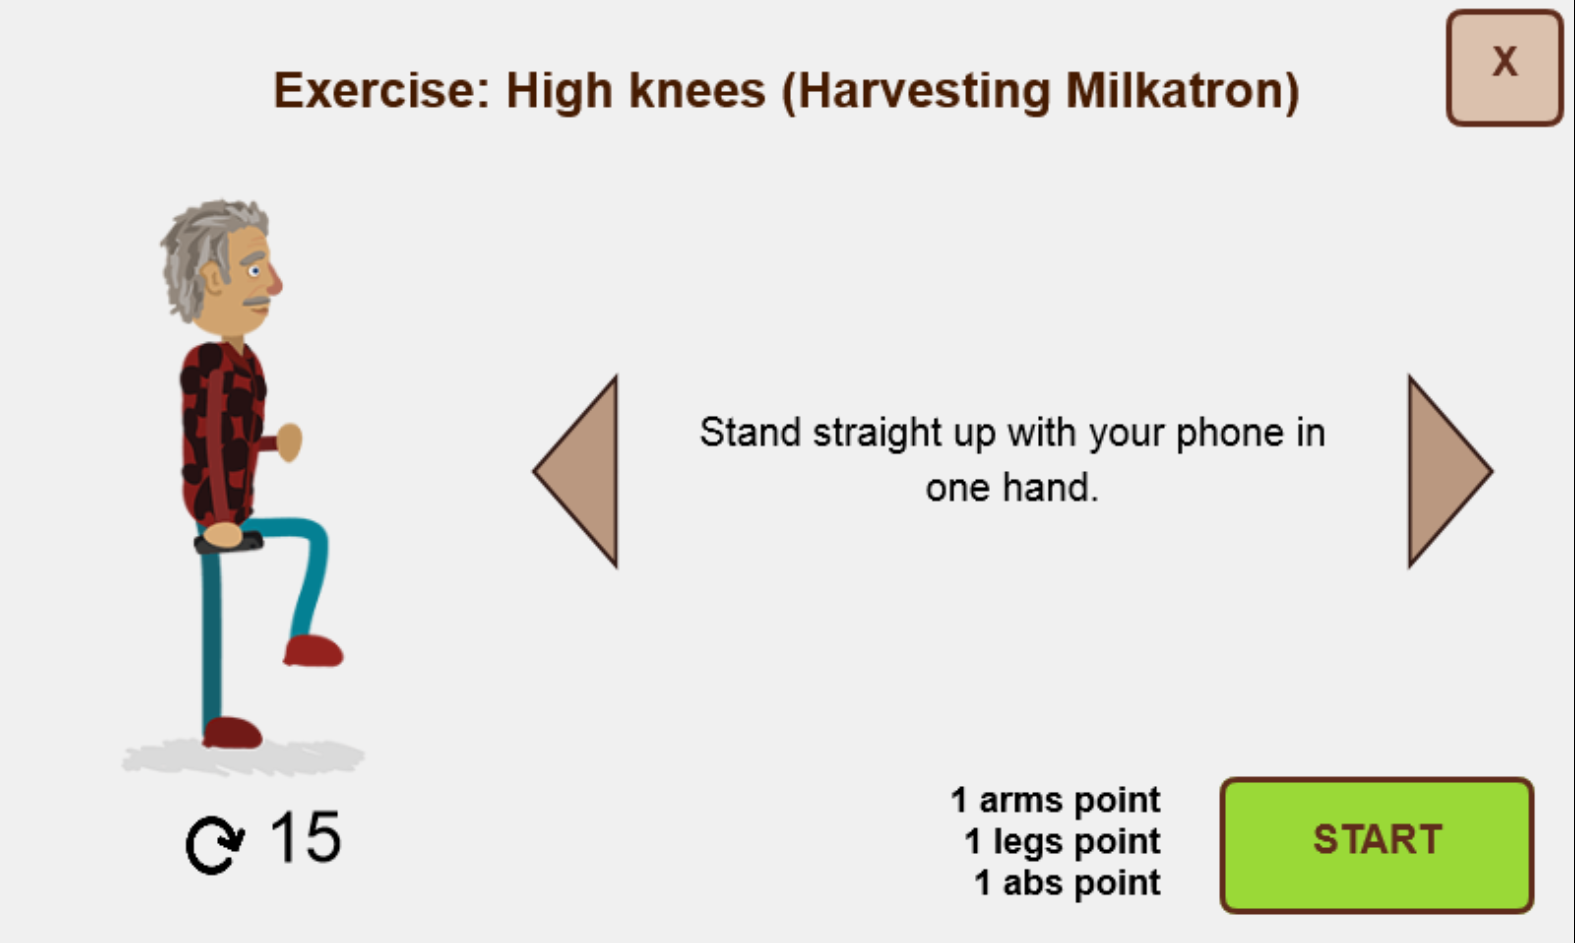
\includegraphics[width=0.80\textwidth]{images/exercise.png}
	\caption{Doing an exercise}
	\label{fig:exercise}
\end{figure}

\paragraph{List of exercises}
A list of current implemented exercises is shown below, categorized by exercises which are measured with the accelerometer and which are timed.
\begin{itemize}
\item Accelerometer exercises %List of accelerometer exercises
\begin{enumerate}
\item Walking
\item Arm stretches
\item Back stretches
\item Sit-ups
\item Dynamic chest stretches
\item Rocket jumps
\item High knees
\item Bear hug crunches
\item Mason twists
\item Wall flying
\item Wall ear touches
\item Wall arm pulling
\end{enumerate}
\item Timed exercises %List of timed exercises
\begin{enumerate}
\item Push ups on knees
\item Push ups
\item Sky kicks
\item Squats
\end{enumerate}
\end{itemize}

\subsubsection{Challenges}
The player has a list of challenges from which he can pick one at anytime and execute that to receive bonus coins. These challenges have an underlying set of exercises that can either be focused on one body part, or they can be a complete body workout. The mentor will explain about that. Challenges are proposed to the player as an appealing task in the game, for example to make a spaceapple pie for your neighbouring Yeowoman that is ill. The player would have to perform some exercises that would be needed to get the ingredients for the space pie, and by doing that he would have completed a workout without noticing. The mentor will inform the player of that afterwards, to raise awareness.
\\\\
You can pick a challenge from the list of available challenges, and you can start it only when you have the required items. These items are used when you do the challenge, so you will not be able to get them back once you have started. After starting the challenge the items are subtracted from your inventory and you can do the required exercises, one at a time. This can be paused anytime, but you will not be able to do any other challenges in the meantime.
\\\\
A screenshot of what an active challenge looks like is shown in Figure~\ref{fig:challenge}.

\begin{figure}[h]
	\centering
		
\includegraphics[width=0.80\textwidth]{images/challenge.png}
	\caption{Doing a challenge}
	\label{fig:challenge}
\end{figure}

\paragraph{Example challenges}
In the current version $8$ challenges are available:
\begin{itemize}
\item Space forest walk
\item Space apple pie
\item Space cookie
\item Woolysocks
\item Carrot pie
\item Apple Sweater
\item Carrot Rocket
\item Strawberry milkshake
\end{itemize}

\subsubsection{Money}
When the game begins the player is provided 150 coins to start developing his farm. After that first allowance he can earn more money by harvesting or by completing challenges. There is also a daily bonus, to reward the players for getting back every day. There might be an occasion, when your crops have died and you have no money nor items left. In that occasion there is a free challenge, which lets you walk around for a while, and which gives you enough money to make a small start again.

\subsubsection{Cloning}
Each type of crop has a name, a cost, a revenue that it yields when harvested and the time it takes for it to grow. Plants will only last one harvest and have to be harvested soon enough (e.g. 12-36 hours, depending on their level), or they will rot away. Trees last multiple harvests.
\\\\
Each type of livestock has a name, a cost, a revenue it yields when exploited and the time it takes for it to be ready (for example milking a Milkatron every 6 hours will produce a bottle of milk and 100 coins). In contrast to the crops, livestock will always stay, it will not die when you don't feed it. To get revenue from livestock, you have to feed them and after a while you will be able to exploit them.
\\\\
All sorts of crops and livestock have a specific exercise attached to them, which the user has to perform to harvest it. The name of the exercise, a preview of the execution, and the amount of experience points it yields are shown on the details screen of the crop or livestock.
\\\\
A screenshot of what the cloning view looks like is shown in Figure~\ref{fig:cloning} and a list of available crops and livestock is shown below.

\begin{figure}[h]
	\centering
		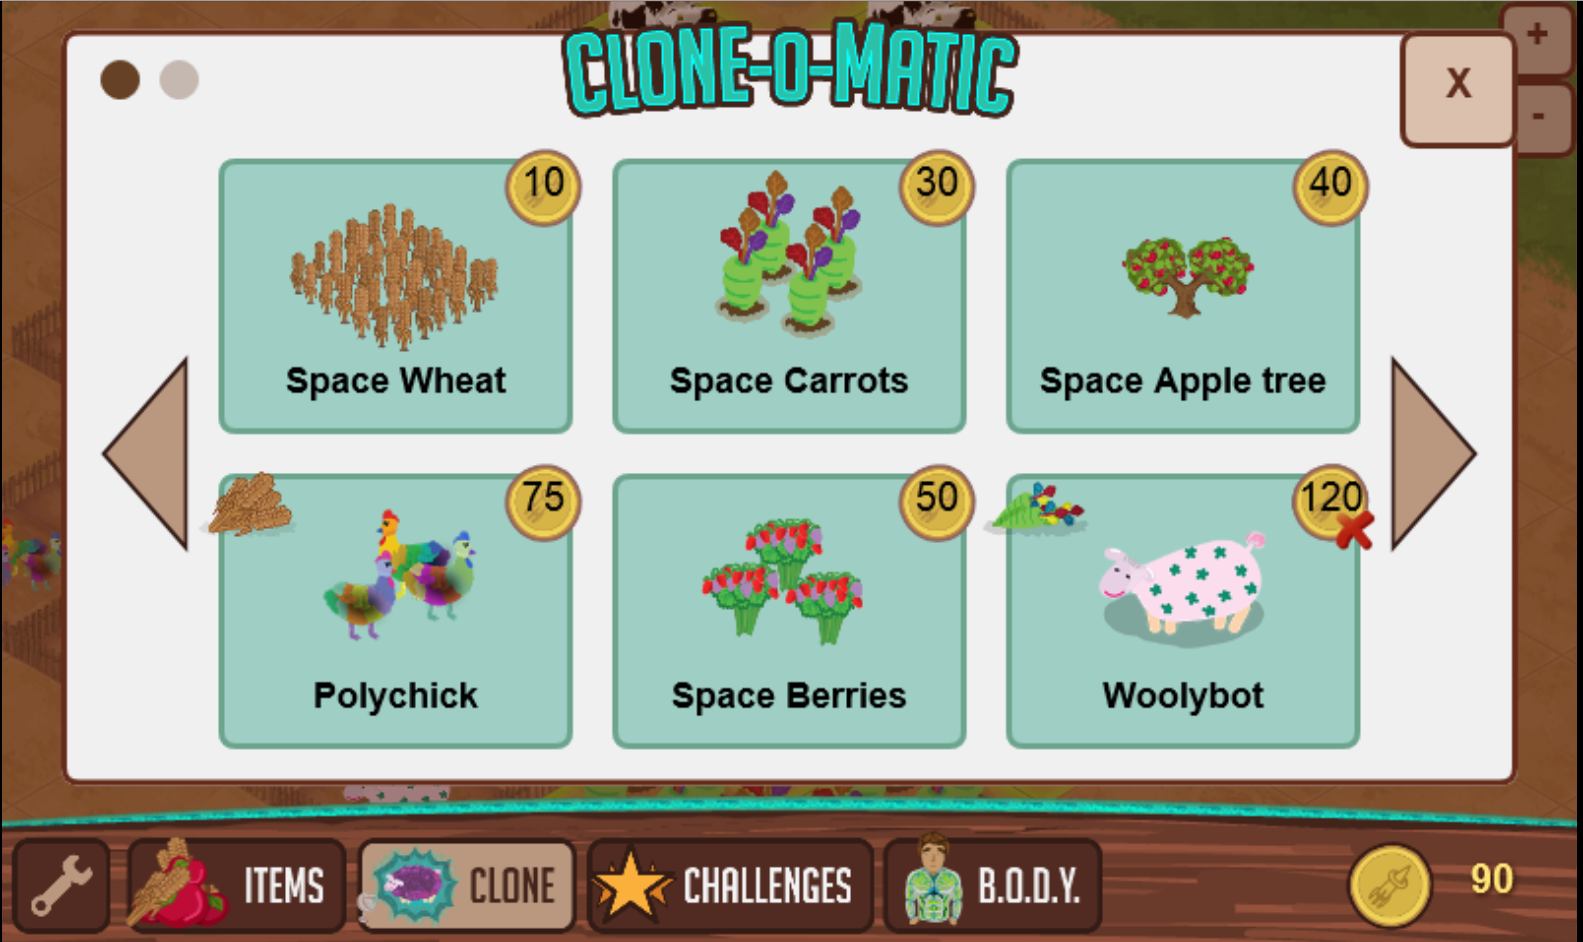
\includegraphics[width=0.80\textwidth]{images/cloning.png}
	\caption{Cloning crops / livestock}
	\label{fig:cloning}
\end{figure}

\paragraph{Available crops (cost, time to grow [minutes], revenue of single harvest, number of harvests)}
\begin{itemize}
\item Space Wheat (10, 10, 15 + 1 space wheat, 1)
\item Space Carrots (30, 45, 50 + 1 carrot, 1)
\item Spaceapple tree (40, 20, 25 + 1 space apple, 3)
\item Space Berries (50, 90, 75 + 1 space berry, 1)
\item Diamond Spirulina (70, 120, 35 + 1 diamond, 3)
\end{itemize}
\paragraph{Available livestock (cost, time to get ready for exploitation [minutes], revenue of single exploitation)}
\begin{itemize}
\item Polychick (75, 45, 20 + 1 egg)
\item Woolybot (120, 120, 40 + 1 wool)
\item Piggium (200, 240, 75 + 1 bacon)
\item Milkatron (300, 360, 100 + 1 milk)
\end{itemize}